\section{Preliminary Actions II}

The following section will report on the outcomes contained in the publication that was delivered during the doctorate programme, including personal contributions as respective co-authors: 

\printpublication{masu_how_2019}

\begin{center}
\begin{tabular}{ p{13cm}}
There has been an increased interest in HCI research regarding the possibilities of interactive technology applied to the field of dance performance, particularly contemporary dance. This has produced numerous strategies to capture data from the moving bodies of the dancers and to map that data into different types of display formats. In this paper, we look at the role of interactive technology in dance from a broader perspective, aiming at understanding the needs of dancers and their relation with the audience. To this end, we ran a focus group with ten dancers with expertise in technology. We analysed the focus group using thematic analysis. We discuss the implications for design of our results by framing the role of technology in dance, proposing design guidelines and analysing appropriation and ambiguity in this context.
\end{tabular}
\end{center}

\section{How do dancers want to use interactive technology? Appropriation and layers of meaning beyond traditional movement mapping}

\section{Introduction}
 
In the last decades, interactive digital artefacts have become ubiquitous, and their applications have gradually switched from workplace to everyday lives and culture. This has been identified as third-wave HCI \cite{bodker2015third}. With this tendency, user experience has become central in HCI discourse \cite{wright2005user}. It has also emerged that users tend to appropriate digital artefacts in different ways \cite{dourish2003appropriation}. Consequently, the use and meaning of artefacts might become ambiguous, and potentially open to many interpretations \cite{gaver2003ambiguity}.
In general, understanding the needs of the user has became a fundamental design activity \cite{bannon2011reimagining}, and users started to be involved in the design process using User Centered Design (UCD).

Among the variety of contexts touched by the spread of application areas in HCI, dance has gained an increased attention, (e.g. \cite{fdili2017seeing}\cite{camurri2016dancer}, and for contemporary dance see \cite{dixon2007digital}). From an HCI perspective, technology for dance can be viewed as a system including input (e.g. sensor technology \cite{fdili2017seeing}) and outputs (e.g. display strategies \cite{hansen2013making}). Related studies have analysed dance from a segmented perspective, mainly focusing on movement characteristics or display approaches. 

We argue that contemporary dance is a complex scenario, requiring a multifaceted approach from HCI, which takes into account the different roles of the technology in creating meaning in the overall dance performance. Currently, there is a lack of design research that tackles interactive dance technology design from this broader perspective. Moreover, in the context of digital performance, the audience perspective started to be investigated in the context of computer music \cite{bin2017moment} and audiovisual performance \cite{correia2017role}, but it is still overlooked in the context of the overlap of HCI and contemporary dance. From this, the following research question emerges:
What is the role of technology in contemporary dance, in particular, interactive technology and visualization?
A secondary objective is to understand 
how that role influences the dancers' communication with the audience. With communication, we mean the communication from the performers to the audience, and the audience's understanding of that communication. Audience participation (communication from the audience to the performers) is out of scope for this study; it is in itself a vast topic that merits a separate study.

In this study, we start to address the identified gap in research by directly questioning dancers. This manuscript presents a focus group with ten dancers and proposes design guidelines based on the analysis of the respective results. The focus group was organised around the following topics: communication to the audience; the role of technology in dance performance; in particular: the role of input technology; and the role of visuals.  

Our results suggest that dancers want to stimulate the audience without imposing one explicit meaning and technology is a co-creator of the performance, that imposes a certain level of initial conditioning of the very logic of the works, that dancers/choreographer need to appropriate to adapt (using different strategies) to create the performance. Moreover, our participants stated that most of interactive technology is too illustrative and diminishes the multilayered complexity of performances, this issue can be overcome using different interaction strategies.

%The design guidelines described in this paper represent a novel contribution to the area of interactive technology for dance design, this contribution points out new design direction. mainly A novelty of this study  performed co-design activity in the very initial stage of the project, without  any conceptual design.

%The rest of the paper is organized as follows: section 2 presents related works in the field of interactive dance technology design particularly focusing on design strategies and the role of sensors and visuals; section 3 describes the focus group and the results; section 4 discusses the design implications of our findings; finally, section 5 concludes by pointing out future steps in the project and future works in general.
 
 
% \section{Literature review}

% \subsection{Interactive Technology for Dance: a state of the art}
 
% The use of interactive technologies in contemporary dance already has a long and established tradition. One relevant example is the work of Mark Coniglio with MidiDancer (1989), a software that allowed a performer to control music \cite{Troikaranch}. A more recent example is the work of Frieder Weiss with the system EyeCon (2004), which allows movement to control several aspects of a performance \cite{wechsler2004eyecon}. Dance artists, researchers and educators have been extensively exploring interactive digital technologies in workshop and rehearsal situations \cite{dinkla2002dance}, and in public performances and installations \cite{latulipe2010exploring}. 
% Different types of inputs can be used to obtain the respective dance data sets. Alaoui and colleagues \cite{fdili2017seeing} for example distinguish among (i) positional data which are retrieved by employing motion capture systems; (ii) movement dynamics (such as acceleration/deceleration), which are recorded by means of inertial sensors; and (iii) physiological information, which can be obtained from biosignal sensor technologies.
% %However, these categories do not include all sensor technologies employed in interactive dance settings. For example, pressure sensors have been used in dance education \cite{grosshauser2012wearable}.  

% Data collected through input technologies has mostly been used to obtain insights from the dancer's body at the dancer's body, resulting in sonification \cite{alborno2016interactive}, visualisation \cite{hansen2013making}, and/or interaction with any other choreographic elements (e.g. scenic design \cite{vincent2018notation}, light design \cite{bouger2010interview}, costumes \cite{birringer2009wearable}). Technological artefacts, which provide the tools for such interactions, used different mapping strategies spanning from direct mapping \cite{wechsler2004eyecon} approaches to agent-based methods \cite{downie2005choreographing}. Visualization strategies include visualization of moving data \cite{barker2018moving}, and visualization of movement qualities \cite{fdili2017seeing}, or more complex visualization of features extracted using different layers of anaysis \cite{camurri2016dancer}. % and practitioners/artists using data art and digital performance (e.g. Choreographic Coding Labs/ Motionbank \cite{mbank}).
%  However, the mentioned studies tackle specific aspects of dance. It appears the systemic perspective of the role of technology in dance is currently overlooked in HCI literature. Therefore, there is a lack of high level design context-related guidelines. 

% %For example, recently pre-recorded data have been used to generate graphics synchronised with animated skeletal representations of the movements using machine learning strategies \cite{ravet2016}.


% \subsection{Designing digital artifacts in the third-wave HCI}

% \subsubsection{Appropriation and ambiguity}
% Within the context of third-wave HCI, where our study is situated, researchers started to investigate the creative uses of interactive digital artefacts \cite{bodker2015third}. In this perspective, artefacts can be used in ways that the designer did not  expect \cite{dourish2003appropriation} and the technology can assume multiple and adaptive meanings. Users appropriate the technology by imposing their own meaning. Dix defined appropriation as ‘’improvisations and adaptations around technology’’ \cite{dix2007designing}. Aligned to this idea, Dourish proposed that to foster appropriation, design should aim to support multiple perspectives on information \cite{dourish2003appropriation}. These multiple perspectives reflects the idea of ambiguity.
% Gaver studied ambiguity in interaction design, proposing different perspectives: ambiguity information; of context as different contexts give different meanings to technology; and of relationship between each user and the artefact \cite{gaver2003ambiguity}.
% These perspectives has been used in artistic branches of HCI, such as music \cite{zappi2014dimensionality} and audiovisual installations \cite{masu2016beatfield}, but are currently unexplored in dance. 

% \subsubsection{User-Centered Design}
 
% UCD is ``a term to describe design processes in which end-users influence how a design takes shape" \cite{abras2004user}. In this perspective, the design process should involve the user to understand their needs in relation to the use of the technological artifact \cite{bannon2011reimagining}. This approach has been successfully used in third-wave HCI, particularly in artistic branches of HCI, for instance to design new musical instruments \cite{turchet2018co}, audiovisual tools \cite{correia2017avui}, and music pedagogy that rely on music and movement \cite{core2017designing}.
% %This approach has been adopted in HCI oriented sound and performance art. For instance ucd has been used to investigate the potential of sonic interaction in personal usage scenario \cite{tanaka201311}. For instance, participatory approaches have also been used to design specific artefacts, such as musical instruments \cite{turchet2018co}, or audiovisual toolkits \cite{correia2017avui}. Core and colleges \cite{core2017designing} adopted participatory approaches to design pedagogical tools for young children that combine music technology and movement.
% Within the area of dance technology, UCD is still generally unexplored, although, in recent years some projects started to involve users in the design process. %Nevertheless, these examples did not research about the role of technology in dance performance.
% For instance, Schofield et al. used workshops to involve teenagers in the design process of an digital artefact for dance performance \cite{schofield2013trigger}. 
% Alauoi and colleagues also involved dancers in the design process of an interactive system based on movement qualities \cite{alaoui2013chiseling}. Another example can be found in a project by Landry and Jeon who involved dancers in the design of an audio-visual system \cite{landry2017participatory}. %They involved the dancers only after that a first prototype was already implemented. 
% What distinguishes these approaches from ours is that they involved participants only after some initial conceptual design or prototype, while we involved dancers in the earliest design stage.

%Despite being valid in defining technological specifications and producing valid artefacts, the studies mentioned above started the design process either with a clear technology, or choreography in mind. Therefore lack of a general understanding of the role of technology within the context of use.

\section{The Study}
To address our research question about the role of interactive technology in dance, and how dancers aim to communicate to the audience, we organised a two-day workshop with dancers, composed of a series of design exercises, including a focus group.

%To address our research question regarding the role of technology in dance, with the involvement of dancers, we organized a two-day co-design workshop. The workshop consisted of a series of design exercises, including a focus group. For the scope of this paper, we will present and analyse the focus group component of the workshop.

\begin{figure*}
\centering
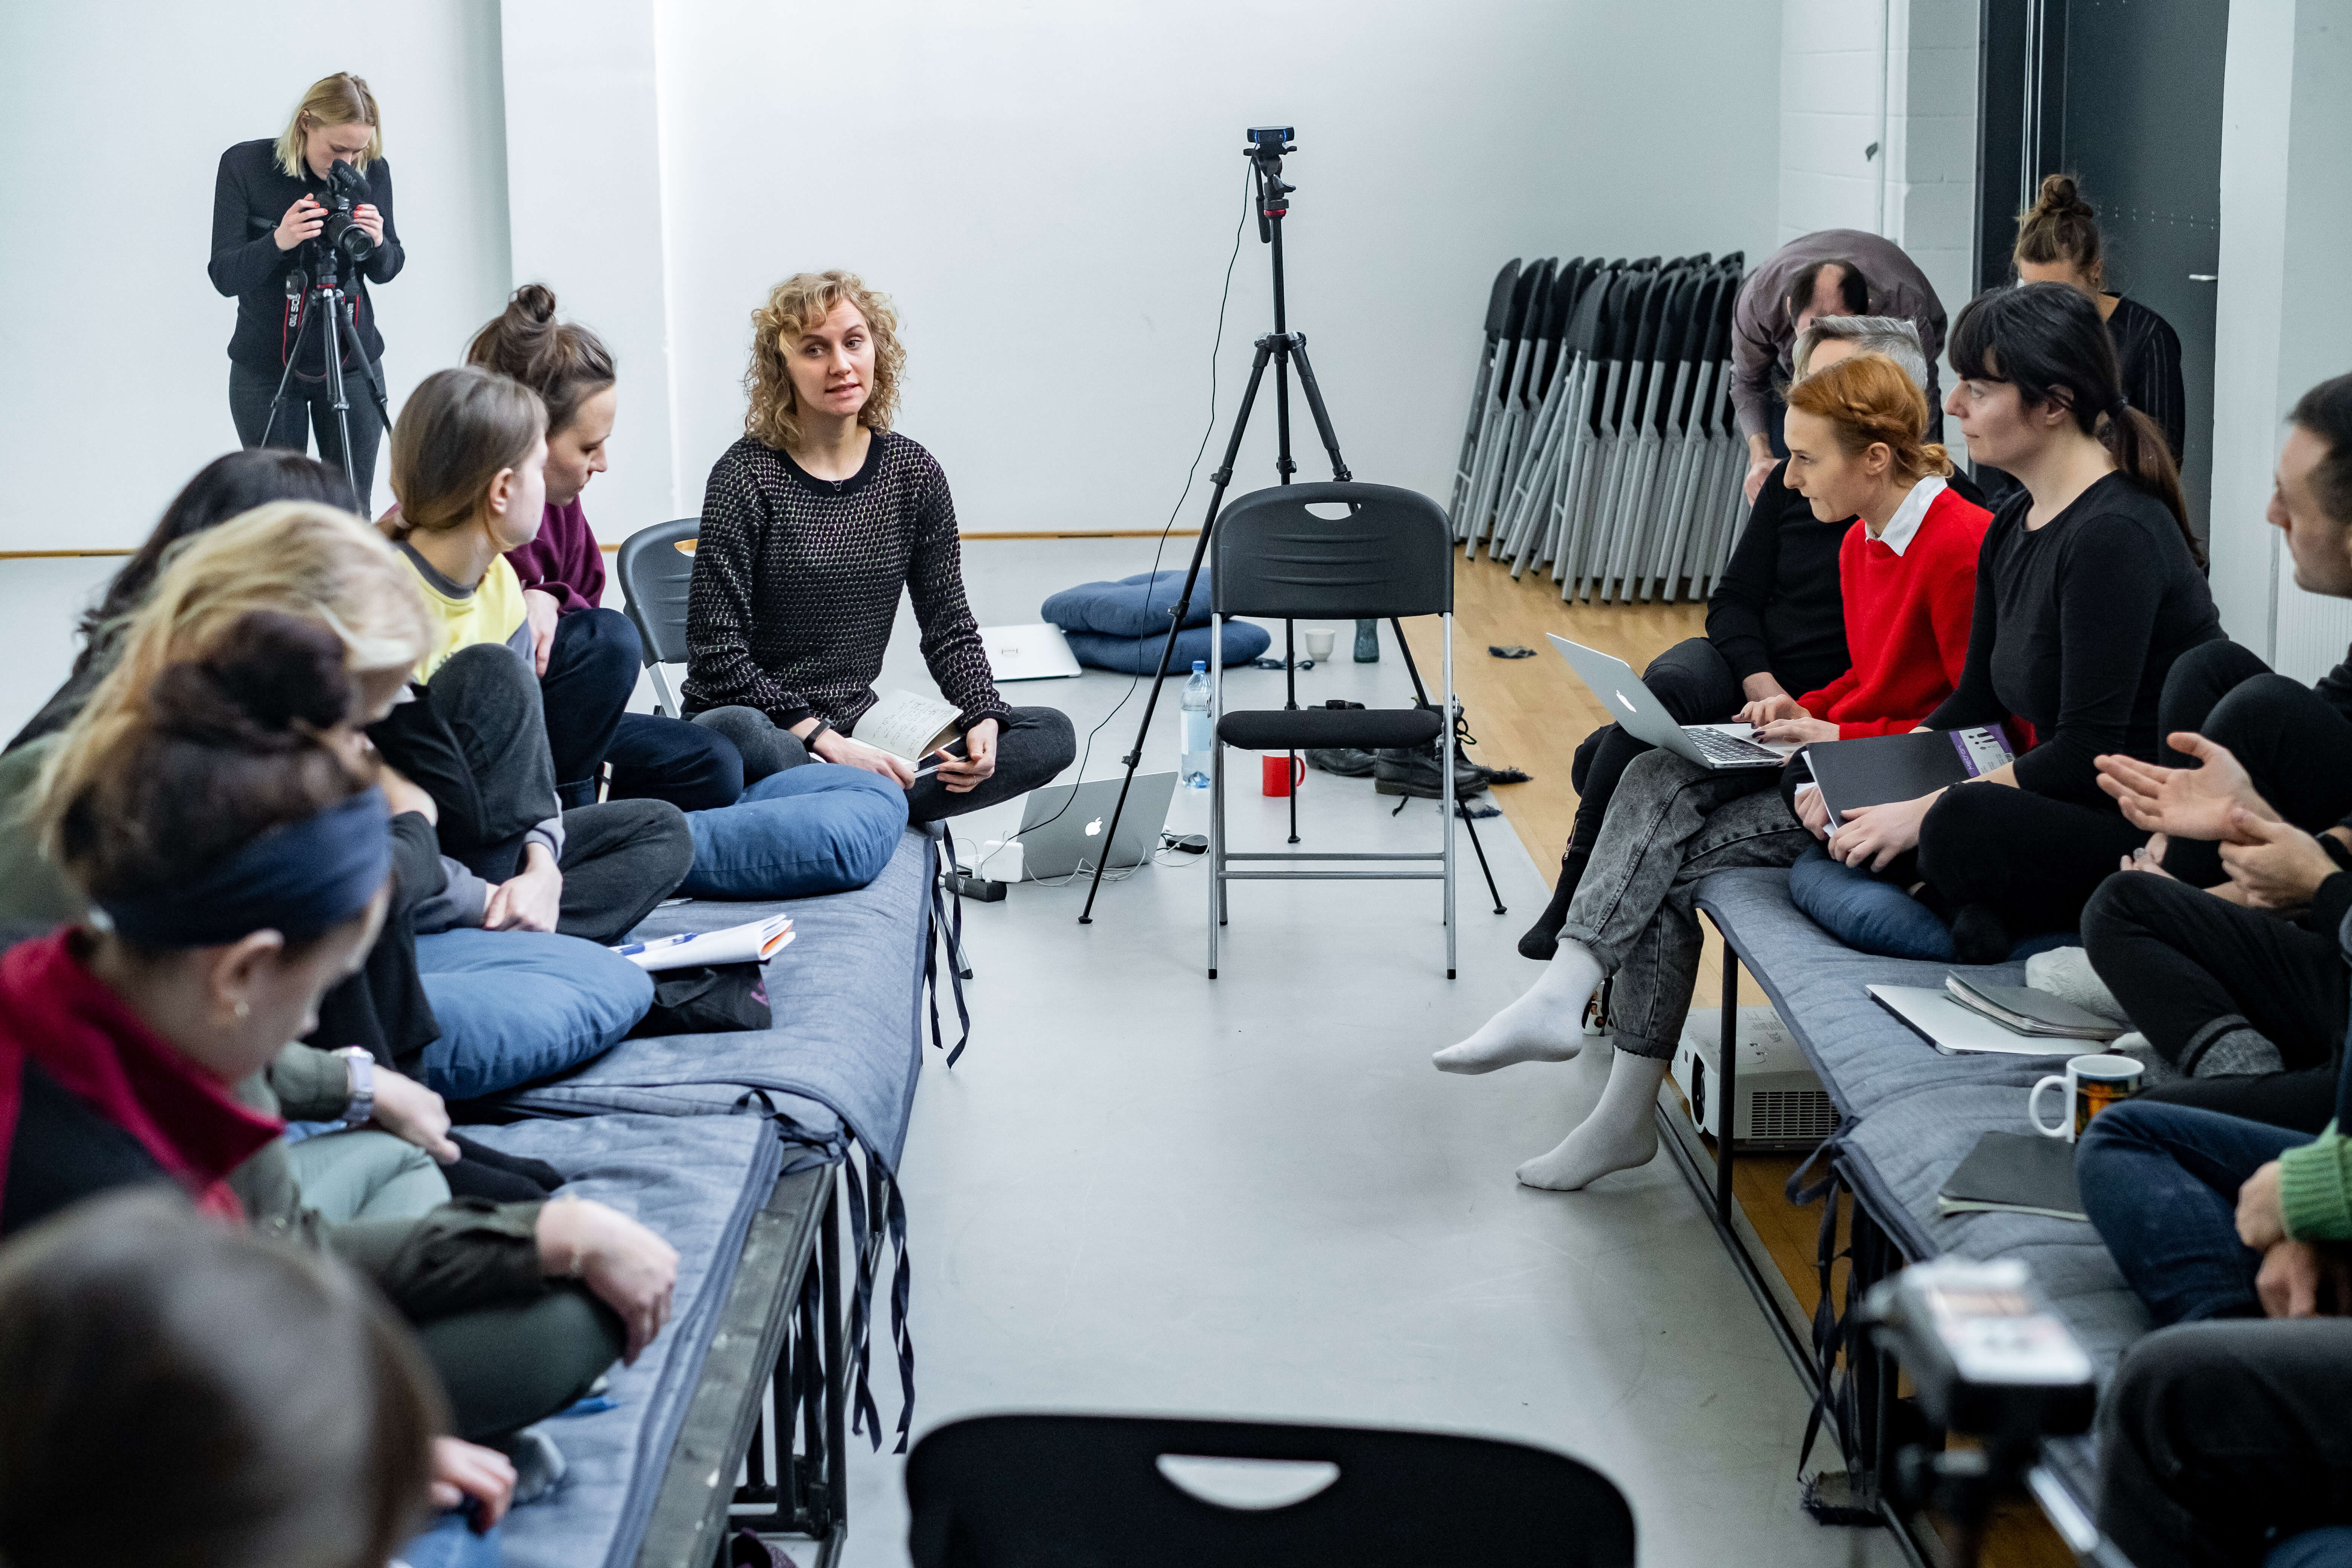
\includegraphics[width=0.9\textwidth]{Chapters/Figures/preliminary_actions/STL_focus_group_optimized.jpg}
\caption{The setting of the focus group.} \label{fig1}
\end{figure*}
%\subsection{The focus group}
%\subsubsection{Participants} 

The participants were selected using an open call, disseminated through mailing lists related to contemporary dance. Ninety-two dancers applied to the call (73 female,  19 male). Each candidate was independently evaluated by six members of our team, according to i) their Curriculum Vitae as dancers, ii) previous experience with technology in dance and iii) motivation and expectations regarding the workshop. Finally, the scores were discussed and moderated. Ten dancers were selected (nine female, one male, from eight countries) and all of them participated in the study. We covered travel expenses and paid a fee for each dancer. Due to the competitive selection, all ten participants had considerable experience in contemporary dance as performers, some of them also as choreographers. All were knowledgeable about the use of technology in dance.

%\subsubection{The focus group} 
The objective of the focus group was to gather data about the role of technology in dance, aiming to identify needs and requirements of dance practitioners. We were also interested in the role technology might have as mediator between dance artists and their audience. Therefore, we structured the focus group around the following four main topics, which align with our research objectives: communication to the audience in dance performance; the role of technology in dance performance; the role of interactive technology; and the role of visuals. The purpose of this focus group was to frame the initial requirements for a future prototyping process. In this way, we followed a UCD perspective, informed by UCD studies presented in the section 2.2: we started by questioning the users about their needs. 
The users (in this case, the dance artists) were involved from an early stage to identify needs and requirements regarding interactive and visualisation technology in dance, which will be the basis for future a in the co-design process. The focus group took place at STL cultural and performance space, lasted for approximately two hours and was audio/video recorded. 

\subsection{Results}

The focus group has been transcribed. It was analysed independently by two researchers using thematic analysis \cite{braun2006using}, then the analysis were cross-checked and harmonised. The analysis produced six themes, each with multiple codes.

\subsubsection{Theme 1: Audience characteristics}

% The first theme concerns the characteristics of the audience. Our participants generally consider the audience intelligent, but also unpredictable. 
% \textbf{\textit{1.1 Audience is intelligent.}}  The first characteristic is that { the audience is intelligent} P8 -moreover, our participants aim to do a { performance for the most intelligent person in the audience} P9.
% \textit{\textbf{1.2 Audience is unpredictable. }}There is uncertainty about the audience: \textit{you really never know who’s sitting in this audience} P2, also the audience members may have an unexpected response P7. %\textit{\textbf{1.3 Audience as abstract individual.}} Our participants tend to consider the audience in abstract terms as an { abstract individual} P.3, an abstract persona.
% \textit{\textbf{1.3 Audience as a close human. }}Finally, there is also a level of closeness with the audience \textit{ It’s a little bit like the creating this human moment of sharing something common, of human to human} P8.

The first theme concerns the characteristics of the audience. Our participants generally consider the audience intelligent, but also unpredictable. 1.1 Audience is intelligent. The first characteristic is that the audience is intelligent P8 – moreover, our participants aim to do a performance for the most intelligent person in the audience P9. 1.2 Audience is unpredictable. There is uncertainty about the audience: you really never know whos sitting in this audience P2, also the audience members may have an unexpected response P7. 1.3 Audience as a close human. Finally, there is also a level of closeness with the audience Its a little bit like the creating this human moment of sharing something common, of human to human P8.

\subsubsection{Theme 2: Communicate with the audience}
Several aspects concerning the communication with the audience emerged. 
\textbf{\textit{2.1 Not impose one specific meaning to the audience.}}
Relying on the fact that the audience is intelligent, the performance should not impose one specific and { didactic} P2 or { prescriptive} P3 perspective, rather create { multi layers of meaning} P5 and information P9.
Dancers aim at not being didactic and at not controlling the audience, even promoting provocative strategies such as deliberately causing confusion ({ un-focusing} P.6). Dancers also do not feel the need to { teach} P2, but prefer to { articulate the performance} and { balance the clarity}, without overexposing an idea P3. 
\textbf{\textit{2.2 Shared experience with the audience.}} 
Relying also on the notion of closeness, our participants aim at creating a sense of { togetherness} P9 with the audience.
The moment of the performance has been described as a shared { intimate} P9 experience between artists and audience, { together [...] and in synchrony} P6 with the audience.  
\textit{\textbf{2.3 Create safe environments for the audience.}} Our participants aim to create { safe environments} P 5., spaces of intellectual freedom where the audience { can come with their own knowledge and their own understanding.} P6. 
\textit{\textbf{2.4 Considering the audience during the creation process.}} In order to check { the clarity of my idea} P3 some of our participants invite audience during the rehearsal asking for feedback. %Our participants stressed the need of ensure clarity { articulation} P. 3  in providing the information to the audience. 
 
\subsubsection{Theme 3: Technology as co-shaper of the performance}
Technology has specific characteristics, which fosters the dancers to reflect on them during the creative process. In this sense, technology becomes co-shaper of the creation process: { the technology is always creating some [...] setting and then it actually become a dramaturgy} P5. 
\textit{\textbf{3.1 The creative technology}}. The technology is creative: { it's like creative dancers [...], there is also creative technology} P3. This creative technology can { generate creative ideas} P2. Therefore, technology may already have a { dramaturgy} P5. There is an awareness of the duality in technological creativity: { Is it a dramaturgy in the technology itself or is the choreographer that tries to use technology as a dramaturgical tool?} P1. 
\textit{\textbf{3.2 Movements fostered by the technology.}} A technological artifact has an impact on the movements, it imposes  { physical limitation} P3 and proposes new types of
 { technological gestures}  P2.
\textbf{\textit{3.3 The problem of excessive focus on technology.}} The technology should never be the focus of a performance P9. It should be { subtle or invisible} P9. Technology can { mesmerize}, and { fascinate} P.6 the audience, but it should not be used in this manner: there is a sheared need to { express something with it} P3.
\textit{\textbf{3.4 Integration of the technology in the logic of the work.}} As a consequence of 3.3, the technology should be { reflected }P3  and { integrated} P9 in the logic of the performance.
\textbf{\textit{3.5 Hacking.}} Our participants describe the process of using the technology as  { hacking} the system P3, in a figurative sense: dancers are not { using the technology the way that the technology designers meant} P3.  

\subsubsection{Theme 4: The problem of redundancy of information} 
One of the main problems that our participants identified is that technology it is often diminishing the layers of meaning in the performance.
\textbf{\textit{4.1 Technology is illustrative.}}  Technology is { too illustrative, [...] and too connected to what you are doing with movement } P6, for this reason it risks to merely duplicate the body P4 .
\textit{\textbf{4.2 Illustration and meaning.}} The visual output is { too graphic, it’s diminishing the multi-layered meaning} P5. and risks to simply replicate the information P6.  

\subsubsection{\bf Theme 5: Strategies for Interaction} From an interaction design perspective, some good practices emerged. 
\textbf{\textit{5.1 Complex mappings.}} Unclear, divergent, or { independent} mappings from input to output technologies could be used to create { counterpoint} P9 between the dancers and the technology, avoiding more obvious mappings P6.
\textit{\textbf{5.2 Interaction Loop.}} Technology could create a complex mirror that challenges the movement of the body P9, a sort of { feedback loop} P3 that affects the choices or behaviour of the dancer. 

\subsubsection{Theme 6: Strategies for visuals/output: adding layers}This last theme clusters suggestions related to the output of the digital artefact.  \textbf{\textit{6.1 Visualize the structure.}} Expose the { score} before P9 or during P6 a performance might contribute to adding layers of meaning. \textit{\textbf{6.2 Play with time-related elements.}} This might include displaying what { things that happened in the past and [..] resonate [...] in a performance } P9, or { traces and the resonance of the movement} P1 \textit{\textbf{6.3 Alternative sensorial strategies.}} Our participants also suggested to rely on other sensorial channels, such us { kinetic illustration} P5 and { sound} that might be used to { trigger sensation} P10. Moreover, sound is { multi-dimensional in space}, and this characteristics makes sound more similar to movement as compared to visuals P5. \textit{\textbf{6.4 Capture the Intelligence.}} Several aspects of the intelligence of a body could be captured and revealed: e.g. { what's happening in the brain before the movement} P6, { record the thinking process of someone doing something incredibly complex} P2. 

\section{Discussion}

The results of the focus group allow us to address our research question. In addition, we  discuss this in light of the concepts of appropriation and ambiguity and propose guidelines.

\subsubsection{{ \textbf{What is the role of technology in contemporary dance, in particular, interactive technology and visualization}?}
%A secondary objective is to understand how that role influences the communication with the audience.
}
Technology plays a crucial role as co-creator of performances, but it should not be the focus. A piece of technology already has its own preexisting dramaturgy, it imposes specific problems or limitations to the choreographer, which need to be incorporated in the ideas and meanings of the performance (Theme 3). %The impact of technology on the creative process of a dancer or choreographer is so big that, to a certain extent, a
 In order to use technology in a meaningful way that is harmonised with the overall performance, dancers need to appropriate the technology and give it a new meaning that is aligned with the dance piece. A performance should be composed of multiple layers of meaning (Theme 2), and technology should contribute to this multifaceted structure (Theme 4, 5, 6). In Theme 4, it emerged that our participants have had issues with technology when it adopts overly clear mappings, since in this case it repeats the same information of the body creating a redundancy issue.  %of the redundancy of information that it imposes on the performance.
This repetition diminishes the layers of meaning of the performance. Consequently, our participants tend to dislike this characteristic of the technology, as they aim to create rich and multi-layered performances. 
The need of structuring the meaning of a performance is connected to the characteristics of the \textbf{audience}. In Theme 1 it clearly emerged that our participants consider the audience intelligent. For these reason, dancers avoid having one clear meaning in the performance. On the contrary, our participants aim to have multi-layered meaning in the performances (Theme 2). We argue that technology should support this approach. 
%Good strategies for designing interactive technology for dancers could include either creating interactive mirror loops or by adding elements to the performance, for instance i) reveal hidden aspects of the performer, ii) play with time lapses, or iii) exposing structural elements of a performance. In general, one-to-one linear input-output mapping appears not to be fruitful in the context of dance performance, as it tends to visualise elements that are already clear in the movement of the body.

\subsubsection{Appropriation and ambiguity in interaction design for dance} 

Our participants' need for reflecting and integrating technology in the performance reverberates with the design concept of appropriation. Similarly, the need for adding layers of meaning and not imposing one single meaning in a performance resonates in the design concept of ambiguity. 
In Theme 3 it emerges that the dancers' use of interactive technology implies a second creative process, whose outcome is a performance. During this process, the dancers need to appropriate the technology \cite{dix2007designing}. Moreover the idea of layering the information is also similar to the idea of designing for appropriation proposed by Dourish: supporting multiple perspectives on information \cite{dourish2003appropriation}. 
In this sense, there are two faces of appropriation: dancers { appropriate} the technology to create multiple layers of meaning in the performance, and the layers of meaning supports the audience to { appropriate} the content of the performance. 
We argue that an interactive digital  artefact designed for dance performers should take into account this aspect, and not impose one restricted meaning or use. On the contrary, it should support dancers to appropriate it, to include it in the overall meaning of the performance. To this end, the artifact should already have ambiguous characteristics that facilitate the appropriation process, as advocated in \cite{gaver2003ambiguity}, rather then impose one clear usage. In Theme 4, 5, and partially 6 it emerged that ambiguity can be used to build the multi-layered meaning of the performance. Therefore, adding ambiguous elements in the technology (e.g. in the rich and complex mapping possibilities  from input/interaction to output/display) could enable dancers to create those multiple layers of meaning. %It is worth noting how all these strategies do not imply linear mapping, that again reverberates ambiguity.

\subsubsection{Design Guidelines} Our design guidelines are organised around three high-level aspects of interactive technology for dancers:


 \renewcommand{\labelitemi}{$\alph$}
 \renewcommand{\labelitemii}{$\alph$}
\begin{enumerate}
em{\bf Communication with the audience}  (from Theme 2)
\begin{enumerate}
em Technology should not impose one single perspective to the audience
em Technology should contribute to create multiple layers of meaning
\end{enumerate}

em{\textbf{Use and role of the technology}} 
(from Theme 3)
\begin{enumerate}
em Technology should provide space for appropriation, enabling the dancer to give their own use and meaning (facilitate customization might be a possible strategy)
em Technology should be easily included in the dramaturgy of the performance -make it meaningful for the performance and hidden
\end{enumerate}


em{\textbf{Input and output strategies}} 
(From Theme 4, 5, and 6) 
\begin{enumerate}
em Technology should not repeat the information that the dancer is already giving with their movement (avoid overly clear mappings) (Theme 4)
em Technology should have a complex input-output mapping, which might be used to create a loop between technology and dancers (Theme 5)
em Technology should facilitate adding information contributing to the multiple meanings of the performance. For example: (i) showing non visible elements (either inner elements of the dancers or micromovements), (ii) shifting the temporal dimension of the performance (e.g. showing, in time lapses, residuals aspects of movement), (iii) showing the structure (score) of the performance (Theme 6)
\end{enumerate}
\end{enumerate}


\subsubsection{Conclusion} 
Compared to other studies that focus on input, output, or mapping strategies in dance this study extends those studies by providing designers with a higher-level view of the role of technology in the dance context. We advocate that our guidelines can assist in the definition of choices and specifications for interaction design in dance. Methodologically, we adopted a UCD approach from an earlier stage, before any initial conceptual design. Thanks to this, our contribution addresses the role of technologies from a systemic level in the general context of a dance performance. 

To conclude, in this paper we presented a focus group study on the role of interactive technology in dance performance. The participants were ten dancers with a background in dance and technology. The results of the focus group allowed us to frame the role of technology in dance, discuss how this contributes to the communication to the audience, analyse appropriation and ambiguity in this context, and propose design guidelines.
